\chapter{Simulation of $pp$ Collision Events}
\label{chap:simulation}


%from: http://imaginaryinstruments.org/lovelace-analytical-engine/
\epigraph{\textit{[The Analytical Engine] might act upon other things besides number, were objects found whose
fundamental relations could be expressed by those of the abstract science of operations, and which should be also susceptible
of adaptations to the action of the operating notation and mechanism of the engine. Supposing, for instance, that the
fundamental relations of pitched sounds in the science of harmony and of musical composition were susceptible of such
expression and adaptations, the engine might compose elaborate and scientific pieces of music of any degree of
complexity or extent.}}{--Ada Augusta, Countess of Lovelace}

%%%%%%%%%%%%%%%%%%%%%%%%%%%%%%%%%%%%%%%%%%%%%%%%%%%%%%%%%%%%%%%%%%%%%%%%%%%%%%%%%
%%%%%%%%%%%%%%%%%%%%%%%%%%%%%%%%%%%%%%%%%%%%%%%%%%%%%%%%%%%%%%%%%%%%%%%%%%%%%%%%%
%%%%%%%%%%%%%%%%%%%%%%%%%%%%%%%%%%%%%%%%%%%%%%%%%%%%%%%%%%%%%%%%%%%%%%%%%%%%%%%%%

In order to be able to make predictions with which comparisons to the observed data
recorded by the ATLAS data can be made, the need for an accurate simulation infrastructure
arises.
Simulation of the $pp$ collision process must be made in order to estimate predicted
rates of specific SM processes so that, in searches for new physics, one can
construct reliable models of both the \textit{background-only} and \textit{background-plus-signal}
hypotheses; the former including only those processes described by the SM and the latter
including additional BSM physics processes on top of the SM ones.
With both models in hand, tests of compatibility between the data recorded by the ATLAS detector
can be made and quantitative statements about the likelihood of either of the two models can be made.

Simulation of the $pp$ collisions in a general purpose high-energy particle-physics detector
like ATLAS implies a precise knowledge of the underlying physics driving the $pp$ interactions; namely,
the theory of QCD.
In Section~\ref{sec:fact_frag} an introduction to the concepts underlying the simulation of QCD
processes will be given.
The simulation of the physics processes rely on detailed Monte-Carlo (MC) programs for their implementation,
a few of which that are relevant to the work presented in this thesis will be described in Section~\ref{sec:mc_gen}.
Section~\ref{sec:detector_sim} then describes how these MC-based simulations of the underling $pp$ collision processes
are put on the same footing as the recorded data via the accurate simulation of the ATLAS
detector and its response to the $pp$ collision products.

%construct a reliable \textit{background-only} model with which the compatibility of data
%and the \textit{background-plus-signal} model, in which a BSM physics process is additionally simulated,
%can be tested {\color{red}{NEEDS RE-WORDING}}.
%In addition to computing overall rates and kinematics of specific physics processes, an accurate
%simulation of the response of the ATLAS detector to these physics events must also be performed which
%requires accurate knowledge of the detector material as well as its read-out such that these, too,
%may be simulated.

%Physics analyses at ATLAS generally rely on simulations of $pp$ collisions,
%and of particular procecesses such as the production of $W$ bosons, in order to build
%a model of how the known SM processes behave.
%By 

\section{QCD Factorization and Fragmentation}
\label{sec:fact_frag}

\begin{figure}[!htb]
    \begin{center}
        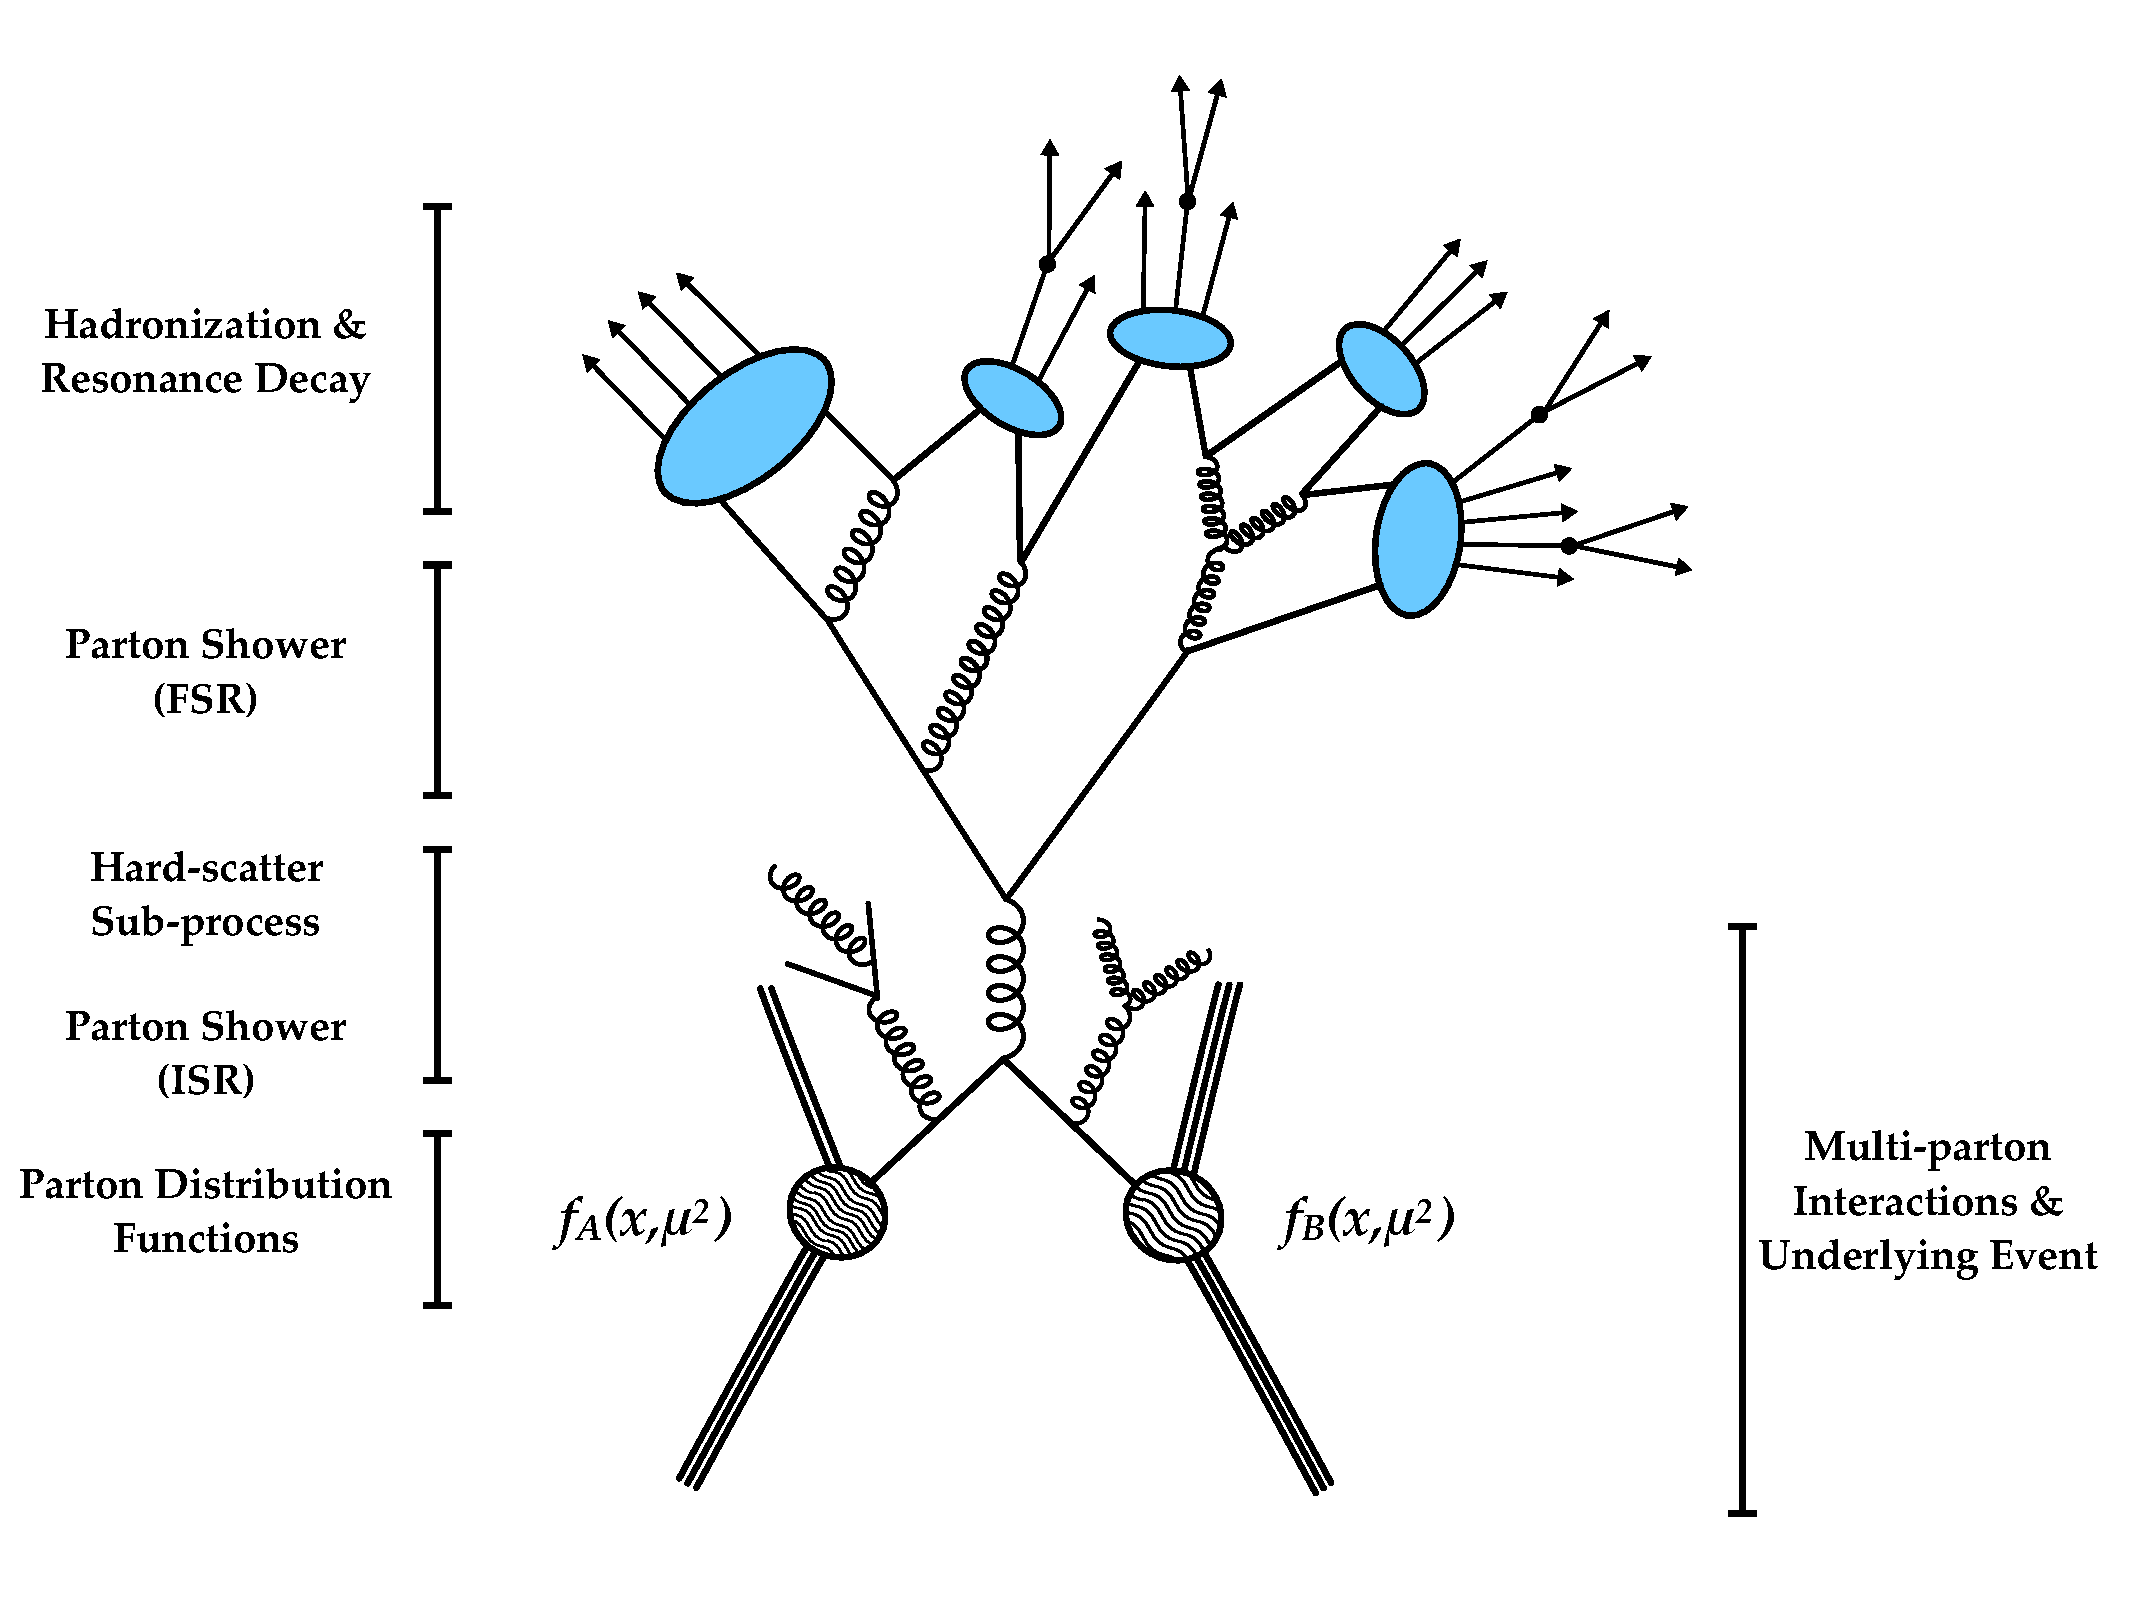
\includegraphics[width=0.75\textwidth]{figures/event_simulation/pp_sim_cartoonPDF}
        %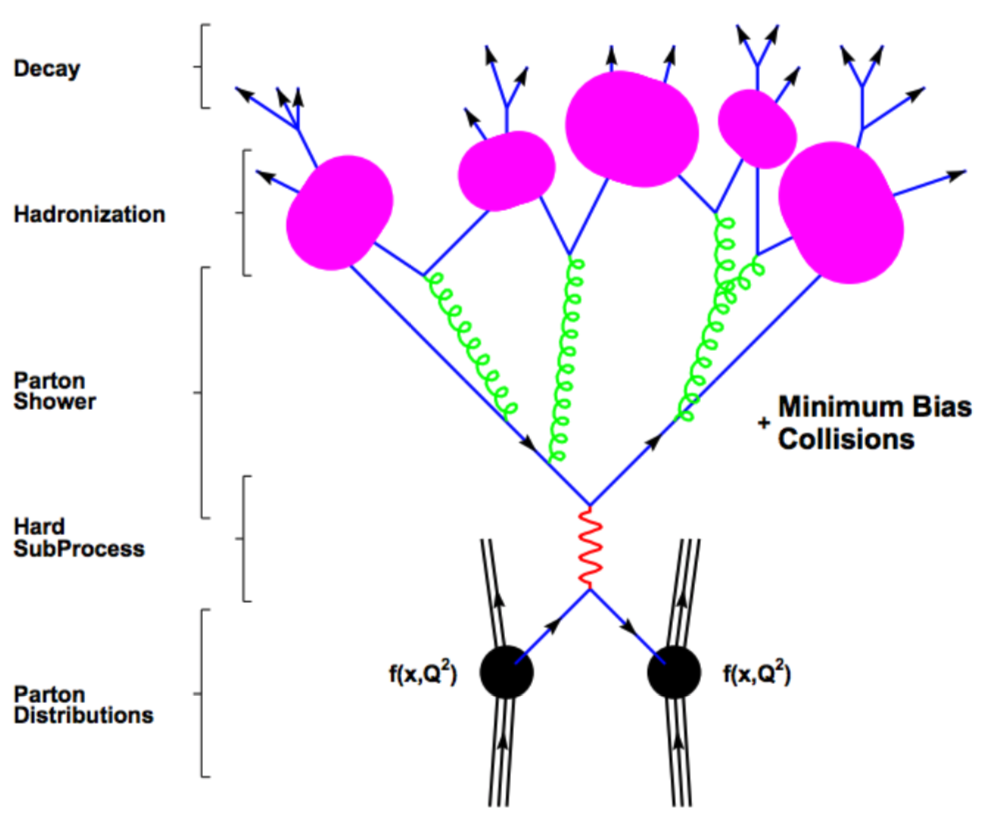
\includegraphics[width=0.6\textwidth]{figures/event_simulation/pp_simulation_steps}
        \caption{
            Cartoon illustration of the Monte-Carlo $pp$ event simulation process.
            The observable color-neutral hadrons at the end result of hardonisation are shown at the
            top, indicated by arrows.
            Example resonance decays could be $K_S \rightarrow \pi^0\,\pi^0$, $\Lambda^+ \rightarrow \pi^+\,n$, or a
            $B$-hadron decay chain.
            The gluons emitted from the incident partons constitute the starting point of the initial state radiation (ISR).
            In order to avoid clutter, the hadronisation of the ISR-emitted gluons and quarks is omitted.
            The blue ovals indicate the location of hadronisation, simulated by phenomenological models as discussed in the text.
        }
        \label{fig:pp_sim_steps}
    \end{center}
\end{figure}

Before simulation of the ATLAS detector response can take place, accurate calculation and simulation of the production of final
state particles as a result of a $pp$ collision must occur.
The steps of such simulation are illustrated in Figure~\ref{fig:pp_sim_steps}.
The breakdown of steps illustrated in Figure~\ref{fig:pp_sim_steps} represent the main characterising features
of QCD, namely: 
\begin{itemize}
    \item Asymptotic freedom (confinement)
    \item Renormalisation group equations (running of scales / scale dependence)
    \item Factorisation (separation of high- and low-energy (perturbative and non-perturbative) regimes)
\end{itemize}

The asymptotic freedom and confinement of QCD state that the strength of the strong coupling, $\alpha_s$, becomes weak at
small distances (high energy scales, $Q^2$) and strong at a large distance.
It is asymptotic freedom that enables the use of perturbative QCD (pQCD) to calculate the hard-scatter (large $Q^2$)
reactions in QCD. Additionally, asymptotic freedom makes the color force dependent on the choice of scale, $Q^2$,
making it necessary to perform computations with respect to a reference scale.
This forces the introduction of arbitrary scales, $\mu$, that are the reference scales enabling the pQCD computations
to proceed but on which physical observables should not depend.
This last requirement leads to the renormalisation group equations that relate pQCD expressions at a given
scale, $\mu$, to physical observables.

The factorisation implied by the above allows us to separate hard-scatter processes from the soft (low energy) parts
of QCD that cannot be calculated perturbatively.
These nonperturbative regimes occur at the characteristic scales of confinment onset, at $Q \sim \Lambda$ ($\sim 200\,\MeV$).
At scales above $m_{\text{hadron}} \sim 1\,\GeV$, the perturbative treatment becomes viable.
%In $pp$ collisions, the parton distribution functions (PDFs) absorb the non-perturbative aspects of the process
%computation and parameterise the probability to find a given parton in the proton holding some fraction of its momentum.
%Being incalculable, the PDFs must be measured in data in separate experiments and are taken
%as input to pQCD calculation, providing the initial conditions of the participating partons at some scale $\mu$ {\color{red}{to which it is evolved using DGLAP}}.
%The remaining computation of the hard-scatter of the initial partons can then be performed using the machinery
%of pQCD.
\begin{align}
    \sigma_{pp \rightarrow X} = \sum\limits_{A,B} \int\limits_0^1 \mathrm{d}x_A \int\limits_0^1 \mathrm{d}x_B \: f_{A}(x_A, \mu_F^2) \, f_{B}(x_B, \mu_F^2) \times \hat{\sigma}_{AB \rightarrow X}(x_A p_A, x_B p_B, \mu_F^2, \mu_R^2)
    \label{eq:pp_xsec}
\end{align}
This factorisation of QCD implies that calculations of $pp$ collision processes take the form of Equation~\ref{eq:pp_xsec},
where the sum runs over the partons of types $A$ and $B$ that exist in the incident protons and that contribute to the hard-scatter process.
The PDFs, $f_{i}(x_i, \mu_F^2)$, absorb the non-perturbabitve aspects of the computation and parameterise the probability
to find a given parton in the proton carrying a fraction of the proton's momentum, $x_i$, evaluated at a given energy scale
$Q^2 = \mu_F^2$.
As the PDFs describe the non-perturbative initial conditions of the partons initiating the hard-scatter processes,
they are incalculable and must be obtained from subsidiary measurements or from altogether
different experiments that are dedicated to their measurement~\cite{Placakyte:2011az,Ball:2012cx}.
The PDFs are measured at specific scales $Q^2$ and are then extrapolated to the energy regime relevant to the physics process
being calculated.
This extrapolation is governed by the Dokshitser-Gribov-Lipatov-Altarelli-Parisi (DGLAP)
evolution equations which evolve the PDFs from one scale to another~\cite{Altarelli:1977zs,Gribov:1972ri,Dokshitzer:1977sg}.
The parton-level cross-section, $\hat{\sigma}_{AB \rightarrow X}$, describes the hard-scatter between the initiating partons
and can be calculated using the machinery of perturbation theory.
Both the PDFs and parton-level cross-section are dependent on the \textit{factorisation scale}, $\mu_F$,
which defines the cut-off scale below which phenomena are absorbed in the PDFs and above which phenomena contribute to the
hard-scatter. 
As with all calculations involving the perturbation theory of QFT, the parton-level cross-section also depends on the
renormalisation scale, $\mu_R$, defining the ultra-violet cut-off scale.
Examples of proton PDFs, measured using data inclusive of $14\,\TeV$ data from the LHC, are provided in Figure~\ref{fig:pdfs_lhc}.

\begin{figure}
    \begin{center}
        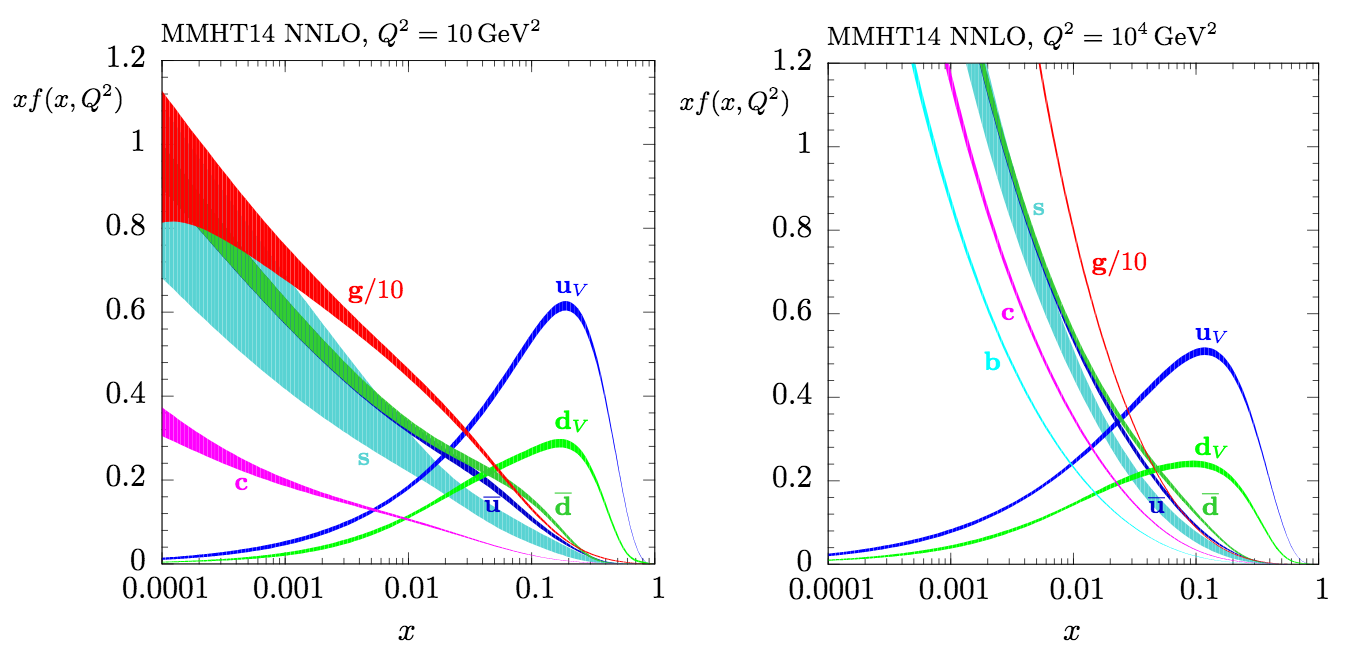
\includegraphics[width=0.9\textwidth]{figures/event_simulation/pdfs_lhc}
        \caption{
            Proton PDFs evaluated at energy scales $Q^2 = 10\,\GeV^2$ (\textit{left}) and $Q^2 = 10^4\,\GeV^2$ (\textit{right}).
            The bands indicate the 68\% confidence-level uncertainty bands.
            The valence-quark components are indicated with a subscript `v' and the sea-quark components without.
            Figures taken from Ref.~\cite{Harland-Lang:2014zoa}.
        }
        \label{fig:pdfs_lhc}
    \end{center}
\end{figure}

The remaining elements of the $pp$ event simulation described by Figure~\ref{fig:pp_sim_steps} are the parton shower (PS)
and hadronisation steps, the latter being non-perturbative and treated with phenomenological models.
The PS simulates the successive emission of quarks and gluons from the partons in the final (initial) state of the
simulated process.
In the collinear factorisation limit, the $n+1$-parton (post-emission) cross-section is related to the $n$-parton (pre-emission) cross-section
as:
\begin{align}
    \mathrm{d}\sigma_{n+1} \approx \mathrm{d}\sigma_n \mathrm{d}P_a(z, q^2) \approx \mathrm{d}\sigma_n \frac{\alpha_s}{2\pi} \frac{\mathrm{d}q^2}{q^2} \mathrm{d}z \, \mathcal{P}_{ab}(z),
    \label{eq:np1_parton_split}
\end{align}
where $\mathrm{d}P_a(z,q^2)$ is the probability that parton $a$ will split into two partons at scale $q^2$, with the parton $b$ carrying the
fraction $z$ of the momentum of the initial parton $a$.
The $\mathcal{P}_{ab}(z)$ are Altarelli-Parisi splitting functions~\cite{Altarelli:1977zs} describing the possible parton branchings: $q \rightarrow gq$, $g \rightarrow gg$, 
or $g \rightarrow q\bar{q}$.
%There are three possible splittings describe by the $P_i$ in QCD: $q \rightarrow gq$, $g \rightarrow gg$, and $g \rightarrow q \bar{q}$.
The PS evolution follows by repeated implmentation of Equation~\ref{eq:np1_parton_split}, leading to arbitrarily many
parton splittings and therefore potentially arbitrarily many particles in the final state.
The basic idea, then, is to evolve the partons as above until they are below a certain energy scale, $q^2 = Q_0^2$, which is the scale
below which the hadronisation process takes place.
In typical PS MC programs, the PS evolution is performed via the construction of the Sudakov form factor,
\begin{align}
    \Delta_{a}(q_1^2, q_2^2) = \exp \left ( - \sum\limits_{b\, \in \{q,g\}} \, \int\limits_{q_2^2}^{q_1^2} \int\limits_{z_{\text{min}}}^{z_{\text{max}}} \frac{\alpha_s}{2\pi} \frac{\mathrm{d}q^2}{q^2} \mathrm{d}z \, \mathcal{P}_{ab}(z) \right),
    %\Delta_{a}(q_1^2, q_2^2) = \exp \left ( - \sum\limits_{b\, \in \{q,g\}} \, \int\limits_{q_2^2}^{q_1^2} \int\limits_{z_{\text{min}}}^{z_{\text{max}}} \mathrm{d}P_{ab}(z,q^2) \right),
    \label{eq:sudakov_form_factor}
\end{align}
which represents the probability that a parton evolves from energy scale $q_1$ to the lower scale $q_2$ \textit{without} splitting.

The PS simulation of the final-state radiation (FSR) operates by following a \textit{forward evolution} whereby partons initially at scale $Q^2$
emit radiation at the scale $q_2$ determined by sampling Equation~\ref{eq:sudakov_form_factor}. This process is repeated and if,
for any of the partons in the final state, the $q_2^2$ value is below $Q_0^2 \approx 1\,\GeV^2$, the shower development is terminated
and hadronisation takes place.
For the simulation of initial-state radiation (ISR), a \textit{backward evolution} occurs wherein the radiation is emitted
by the initiating partons. In this case the final low-energy scale is that of the ancestor partons fragmenting from the PDFs, gaining energy to take part
in the hard-scatter, and the initial energy scale is the high-energy scale of the hard-scatter.
For this reason, the ISR shower evolution is dependent on the factorisation scale $\mu_F$ through
its sensitivity to the value of the PDFs.

As the partons reach the hadronisation scale, the confining nature of QCD takes over and the non-perturbative regime of QCD is reached
once again.
At this stage, the color-neutral hadrons that are observable within the detector take form.
This formation process is described by phenomenological models that capture the general
features of QCD.
The main hadronisation models used in the MC simulation relevant to the current analysis are the
Lund string model~\cite{Andersson:1983ia} and cluster hadronisation model~\cite{Webber:1983if}.
Unstable particles produced as a result of the hadronisation process are also decayed at this point;
in some cases relying on the use of dedicated programs such as \textsc{EvtGen} in the case of $b$-hadron decays~\cite{Lange:2001uf}.

The so-called \textit{spectator partons}, indicated by the outgoing lines from the PDFs in Figure~\ref{fig:pp_sim_steps},
are those partons not directly involved in the $pp$ hard-scatter sub-process.
They may undergo soft interactions, resulting in the underlying event (UE).
The physics processes underlying the UE are driven by low-energy phenomena and must therefore
be simulated using phenomenological modes, in much the same way as the hadronisation simulation.
These models are characterised by tuneable parameters which are optimised by dedicated measurements
and comparisons to observed data in the experiments~\cite{UESim}.
There is also processes of multiple-parton interactions (MPI) in which there are additional,
relatively soft, parton-parton scattering processes in addition to the hard-scatter subprocess.
The processes of UE and MPI result in long-distance QCD color connection effects that lead
to additional radiation of quarks and gluons, also simulated using tuneable phenomenological models
provided by specific MC generators~\cite{Sjostrand:2006za,Butterworth:1996zw}.



%%%%%%%%%%%%%%%%%%%%%%%%%%%%%%%%%%%%%%%%%%%%%%%%%%%%%%%%%%%%%%%%%%%%%%%%%
%%%%%%%%%%%%%%%%%%%%%%%%%%%%%%%%%%%%%%%%%%%%%%%%%%%%%%%%%%%%%%%%%%%%%%%%%
%%%%%%%%%%%%%%%%%%%%%%%%%%%%%%%%%%%%%%%%%%%%%%%%%%%%%%%%%%%%%%%%%%%%%%%%%
%
% MC GENERATORS MC GEN mc gen
%
%%%%%%%%%%%%%%%%%%%%%%%%%%%%%%%%%%%%%%%%%%%%%%%%%%%%%%%%%%%%%%%%%%%%%%%%%
%%%%%%%%%%%%%%%%%%%%%%%%%%%%%%%%%%%%%%%%%%%%%%%%%%%%%%%%%%%%%%%%%%%%%%%%%
%%%%%%%%%%%%%%%%%%%%%%%%%%%%%%%%%%%%%%%%%%%%%%%%%%%%%%%%%%%%%%%%%%%%%%%%%

\section{Monte-Carlo Event Generators}
\label{sec:mc_gen}

There are a handful of MC-based event generators dedicated for LHC physics
and the implementation of the processes described in the previous section and illustrated
in Figure~\ref{fig:pp_sim_steps}~\cite{Buckley:2011ms}.
In the following we reference those relevant to the work to be presented in the current
thesis.

\subsection{Matrix Element Generators}
\label{sec:mc_gen_me}

Matrix element (ME) MC generators provide calculations of the matrix element corresponding
to the underlying $pp$ hard-scatter sub-processes.
They are generally supplemented by separate PS MC generators that perform the subsequent
showering, hadronisation, etc...

\begin{description}
    \item[] \underline{\textsc{MadGraph5\_AMC@NLO}} \cite{MGFive} is an MC event generator providing automated
        computation of matrix elements at LO, with NLO computations aided by the MC@NLO method~\cite{AMCNLO}.
    \item[] \underline{\textsc{Powheg-Box}} \cite{POWHEGBOX} is a library for implementing NLO calculations in
        MC programs using the \textsc{Powheg} formalism~\cite{POWHEGMETHOD} to match the matrix element
        computation to that of the PS.
    \item[] \underline{\textsc{Pythia}}
    \item[] \underline{\textsc{Sherpa}}
    \item[] \underline{\textsc{Herwig}}
\end{description}

%%%%%%%%%%%%%%%%%%%%%%%%%%%%%%%%%%%%%%%%%%%%%%%%%%%%%%%%%%%%%%%%%%%%%%%%%
%%%%%%%%%%%%%%%%%%%%%%%%%%%%%%%%%%%%%%%%%%%%%%%%%%%%%%%%%%%%%%%%%%%%%%%%%
%%%%%%%%%%%%%%%%%%%%%%%%%%%%%%%%%%%%%%%%%%%%%%%%%%%%%%%%%%%%%%%%%%%%%%%%%
%
% DETECTOR SIMULATION
%
%%%%%%%%%%%%%%%%%%%%%%%%%%%%%%%%%%%%%%%%%%%%%%%%%%%%%%%%%%%%%%%%%%%%%%%%%
%%%%%%%%%%%%%%%%%%%%%%%%%%%%%%%%%%%%%%%%%%%%%%%%%%%%%%%%%%%%%%%%%%%%%%%%%
%%%%%%%%%%%%%%%%%%%%%%%%%%%%%%%%%%%%%%%%%%%%%%%%%%%%%%%%%%%%%%%%%%%%%%%%%


\section{Simulation of the Detector Response}
\label{sec:detector_sim}

%Up until the stage of hadronisation, the Monte-Carlo event simulation depends only on the nature of the
%incident beam (i.e. proton beam and bunch structure) and on the beam energy ($\sqrt{s} = 13\,\TeV$).
%These are taken as configuration parameters needed for calculating the hard-scatter sub-process
%and initiating fragmentation.
The end result of the steps discussed above and outlined in Figure~\ref{fig:pp_sim_steps}
is a collection of four-vectors of all stable particles after hadronisation.% and that have the potential to leave detectable
%signatures in the ATLAS detector.
By itself, this collection of particle four-vectors is useful for studying physics processes at
the so-called \textit{truth}- or \textit{particle}-level, allowing one to understand specific
processes without the effects of the ATLAS detector's geometric acceptance and response folded in.

Ultimately, however, one wishes to use the MC simulation to make predictions on the collection of specific physics
processes being simulated.
To use the MC simulated events in this way, they need to be compared to the recorded data and therefore must be analyzed after
the full ATLAS reconstruction process, described in Section~\ref{chap:objects}, so as to ensure meaningful comparisons are made.
%To compare the MC simulation to data, so that one can make meaningful predictions for specific
%physics processes, the output of the MC simulated event generation must be analyzed after the
%full ATLAS reconstruction described in Section~\ref{chap:objects} takes place.
To accomplish this, a detailed \textsc{GEANT4}~\cite{GEANT4} model of the ATLAS detector is used
which includes not only the sensing elements of each of the subdetectors but also includes
simulation of inactive material such as support structures, cabling, and services~\cite{ATLASSim}.
Custom algorithms are developed for each of the ATLAS subdetectors which convert the simulated \textsc{GEANT4}
energy depositions into hits on the corresponding detectors, modelling the detailed nature
of each subdetector's response to incident particles.
For example, the simulation of the MDT drift tubes (Section~\ref{sec:ms}) includes realistic simulation of signal formation as a result of the ion
drift and avalanche evolution as well as a realistic simulation of the response
of the readout electronics that produce the digitized output signals.
The result of the simulation, then, is a set of simulated digitized output signals which
may then be treated by the same reconstruction algorithms used during actual data taking, including the trigger.
The paths of the particle-level and fully reconstructed simulated $pp$ collision events, as well
as the paths of the data events, through the simulation and reconstruction infrastructure are illustrated in Figure~\ref{fig:atlas_sim_structure}.

{\color{red}{How is pileup simulated?}}
%{\color{red}{The computing infrastructure needed for simulation is large...}}

\begin{figure}[!htb]
    \begin{center}
        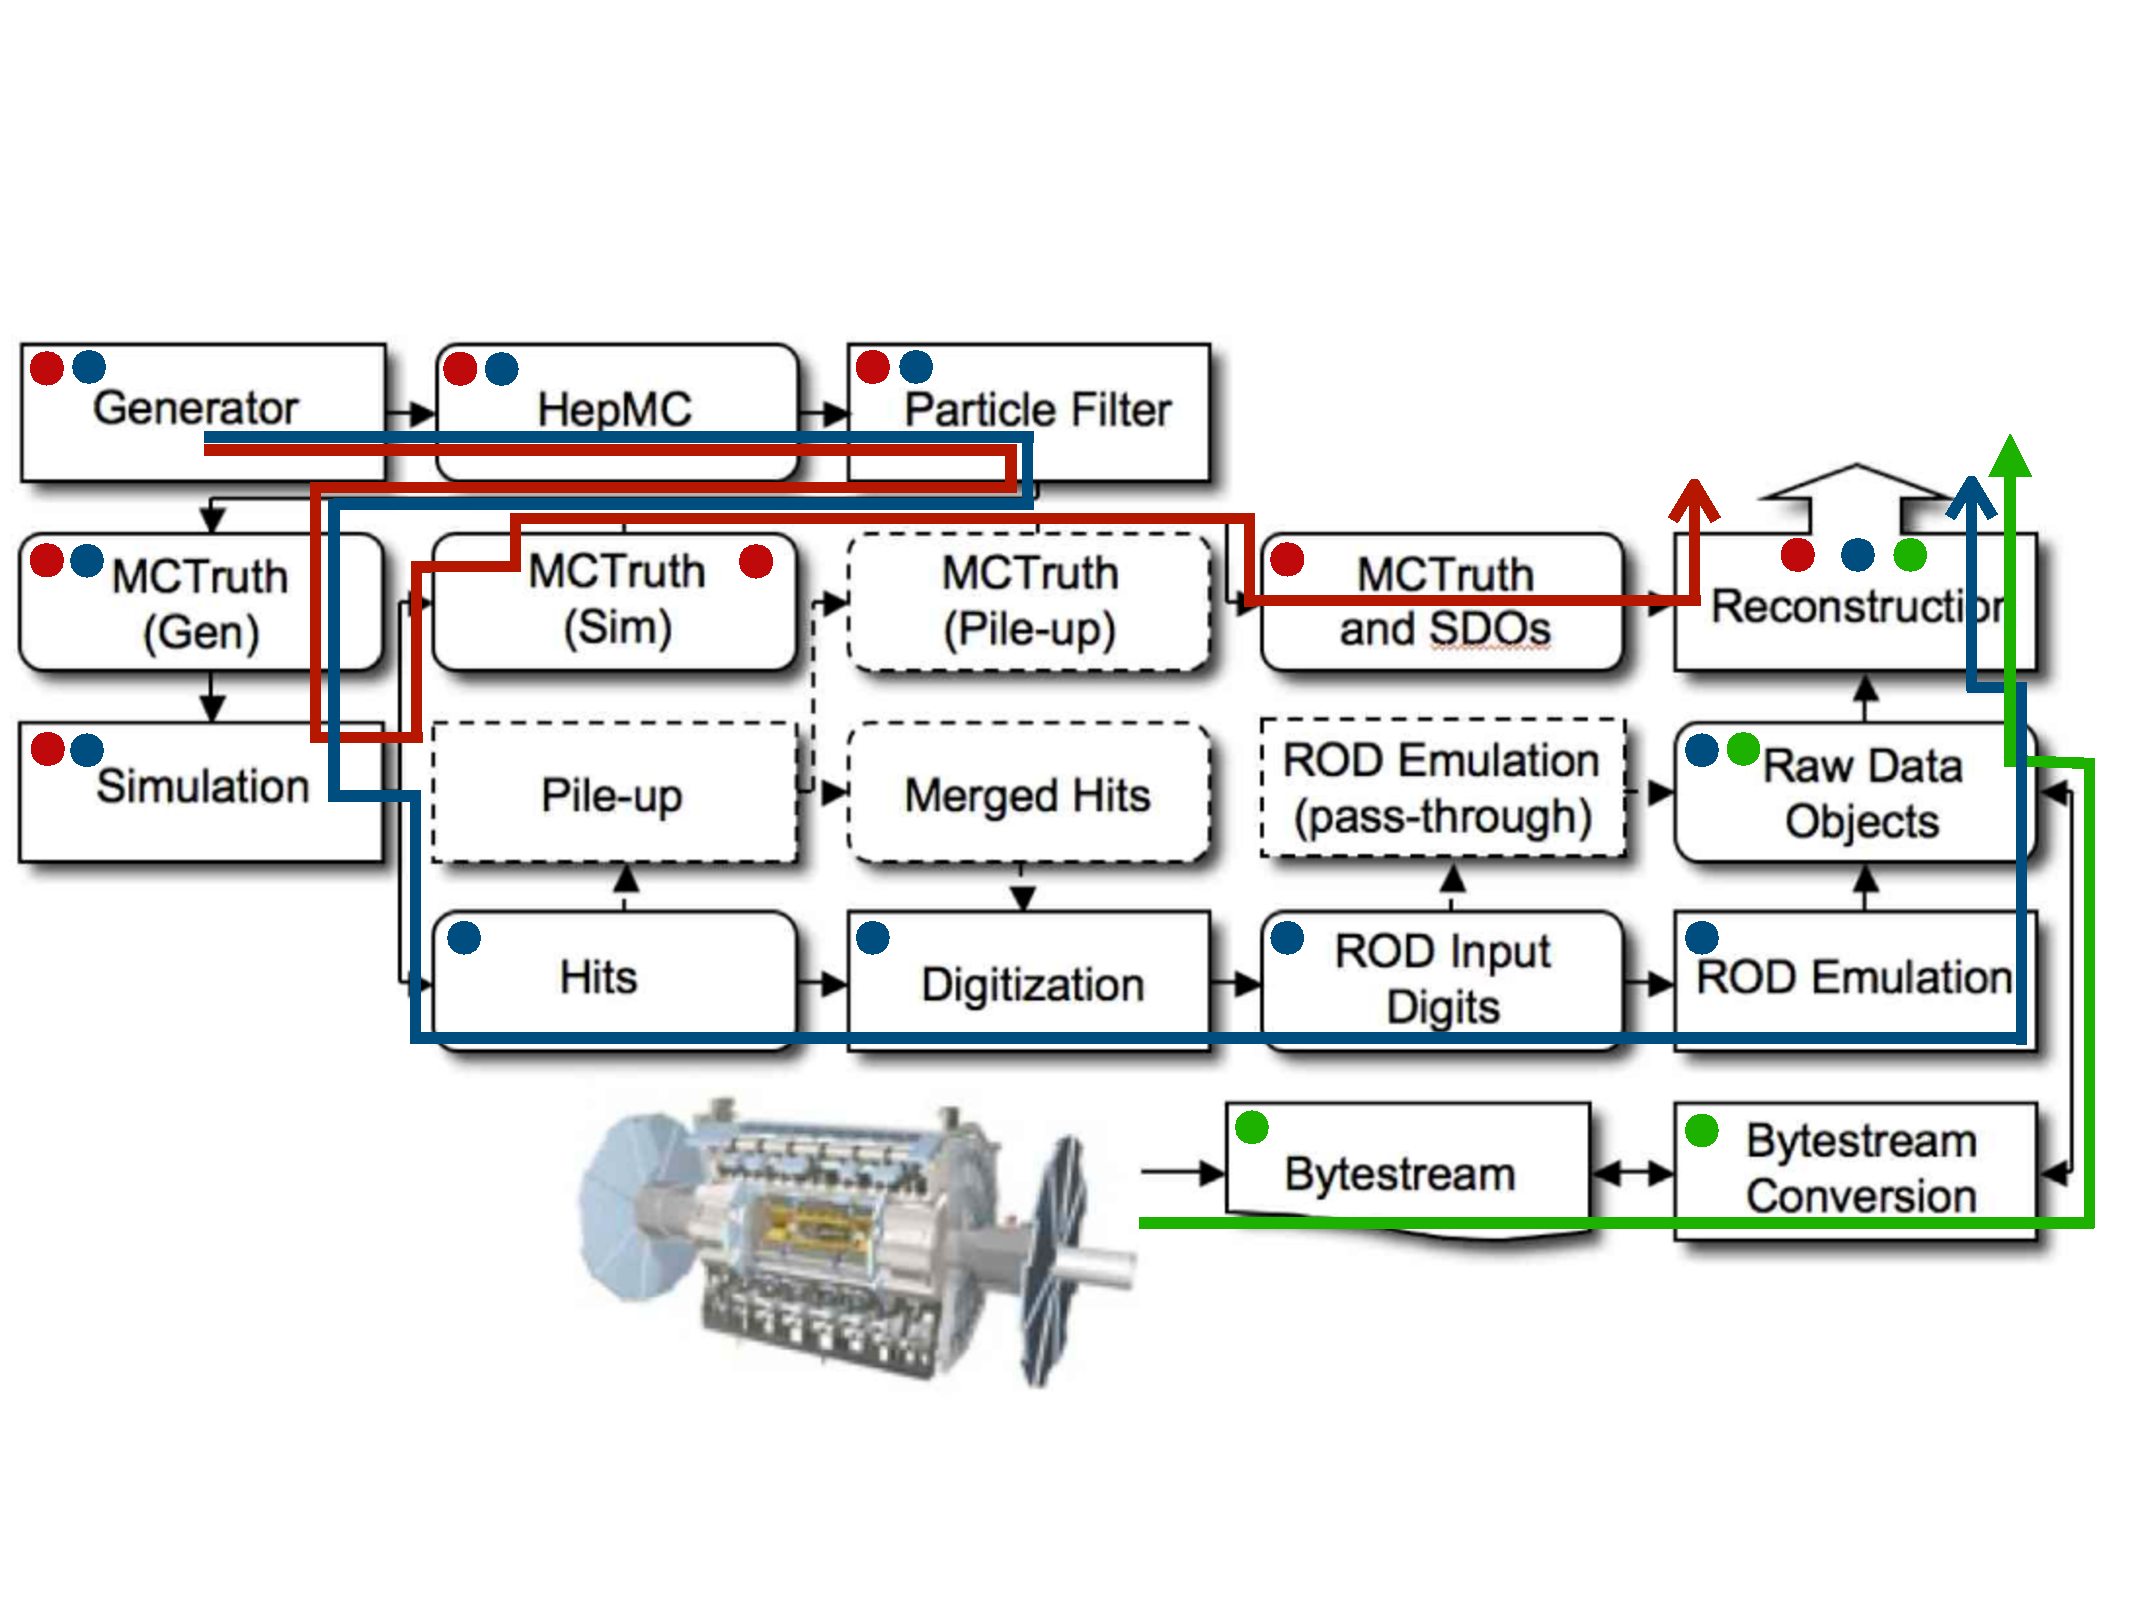
\includegraphics[width=0.85\textwidth]{figures/event_simulation/atlas_sim_structure_arrPDF}
        \caption{
            Paths of the ATLAS $pp$ event simulation, starting from the MC event generation all the way
            to the full ATLAS reconstructed event.
            The red path and markers indicate that of the particle-level (truth-level) events,
            while the blue path and markers indicate that of the fully reconstructed simulated events.
            The green path and markers show the path that real data takes when reconstructed and recorded by ATLAS.
            The acronym SDO (ROD) stands for `Simulated Data Object' (`ReadOut Driver').
            Original figure taken from Ref.~\cite{ATLASSim}.
        }
        \label{fig:atlas_sim_structure}
    \end{center}
\end{figure}
